\RequirePackage{amsmath}
\documentclass[twocolumn, times]{aastex63}
\usepackage[spanish,es-minimal,english]{babel}
\usepackage[utf8]{inputenc}
\usepackage{natbib}
%\usepackage{microtype}
\usepackage{hyperref}
\usepackage{savesym}
\savesymbol{tablenum}
\usepackage{siunitx}
\restoresymbol{SIX}{tablenum}
\usepackage[varg]{newtxmath}
\usepackage{newtxtext}
\usepackage{booktabs}
\usepackage{array}   % for \newcolumntype macro
\newcolumntype{L}{>{$}l<{$}} % math-mode version of "l" column type
\newcolumntype{R}{>{$}r<{$}} % math-mode version of "r" column type

\bibliographystyle{aasjournal}

\newcommand\ION[2]{#1\,\scalebox{0.9}[0.8]{\uppercase{#2}}}
\newcounter{ionstage}
\renewcommand{\ion}[2]{\setcounter{ionstage}{#2}% 
  \ensuremath{\mathrm{#1\,\scriptstyle\Roman{ionstage}}}}
\newcommand\hii{\ion{H}{2}}
\newcommand\Raman{\ensuremath{_{\text{Raman}}}}
\def\th#1#2{\(\theta^{#1}\)\,Ori~#2}

% Chemical formulae
\newcommand*\chem[1]{\ensuremath{\mathrm{#1}}}

\begin{document}
\title{Raman mapping of atomic hydrogen in the Orion Bar and Orion South}
\shorttitle{Raman mapping of atomic hydrogen in Orion}
\author{William J. Henney}
\affiliation{%
  \foreignlanguage{spanish}{Instituto de Radioastronomía y
    Astrofísica, Universidad Nacional Autónoma de México, Apartado
    Postal 3-72, 58090 Morelia, Michaoacán, Mexico}}
\email{w.henney@irya.unam.mx}

\begin{abstract}
  I show that the broad Raman-scattered wings of H\(\alpha\) can be used to
  map neutral gas illuminated by high-mass stars in star forming
  regions. The near wings (\(\Delta\lambda \approx \pm \SI{10}{\angstrom}\)) trace neutral columns Absorption features in the pseudo-continuum at 6634 and
  6663~\AA{} correspond to neutral oxygen far-ultraviolet absorption
  lines at \SIlist{1027.43;1028.16}{\angstrom}.
\end{abstract}

\keywords{Atomic physics; Radiative transfer; Photodissociation regions}
\facilities{VLT:Yepun (MUSE); OANSPM:2.1m (Mezcal)}
\object{M42}
\section{Introduction}
\label{sec:introduction}

Raman scattering is the inelastic analog of Rayleigh scattering by atoms or molecules.  Both processes begin with a radiation-induced transition of an electron to a virtual bound state (non-eigenstate)

non-resonant scattering 
Recently, \citet{Dopita:2016a} identied Raman scattering wings to the
H\(\alpha\) line in the Orion Nebula and a number of \hii{} regions in the
Magellanic Clouds.

\citet{Dopita:2016a} propose that the Raman wings form at the
transition zone near the ionization fronts in \hii{} regions.
However, the total neutral hydrogen column through the ionization
front can be no more than about
\(10 / \sigma_0 \approx \SI{2e18}{cm^{-2}}\), where
\(\sigma_0 \approx \SI{6.3e-18}{cm^2}\) is the ground-state hydrogen
photoionization cross section at threshold \citep{Osterbrock:2006a}.
The Raman scattering cross section at wavelengths responsible for the
observed wings is much lower than this:
\(\sigma\Raman \sim \SI{e-22}{cm^2}\) \citep{Chang:2015a}, meaning that the
Raman scattering optical depth through the ionization front is only of
order \(0.0001\).  A vastly larger column density of neutral hydrogen
is available in the photodissociation region outside the ionization
front, so it is more likely that Raman scattering will occur there
instead, so long as there is sufficient far ultraviolet radiative flux
in the vicinity of the Lyman~\(\beta\) line (\SI{1025}{\angstrom}).

\section{Observations}
\label{sec:observations}

MUSE \citep{Bacon:2010a} observations of the Orion Nebula \citep{Weilbacher:2015a, Mc-Leod:2015b}.

Keck HIRES spectra described in \citet{Henney:1999a} and
\citet{Bally:2000a}. The spectrum I use is of HH~529 base region in
Orion~South. Published results from these data have concentrated on
strong nebular lines, but here I use a small section of the spectrum
in the range \SIrange{6660}{6670}{\angstrom} for reasons which will
become apparent.

\begin{table}
  \centering
  \caption{Wavelength bands used for extracting Raman-scattered light}
  \label{tab:wav-bands}
  \begin{tabular}{lll}
    &&
  \end{tabular}
\end{table}

\begin{figure}
  \centering
  
  \caption{Spatial distribution of Raman-scattered wings in H\(\alpha\)}
  \label{fig:raman-maps}
\end{figure}

\begin{figure*}
  \centering
  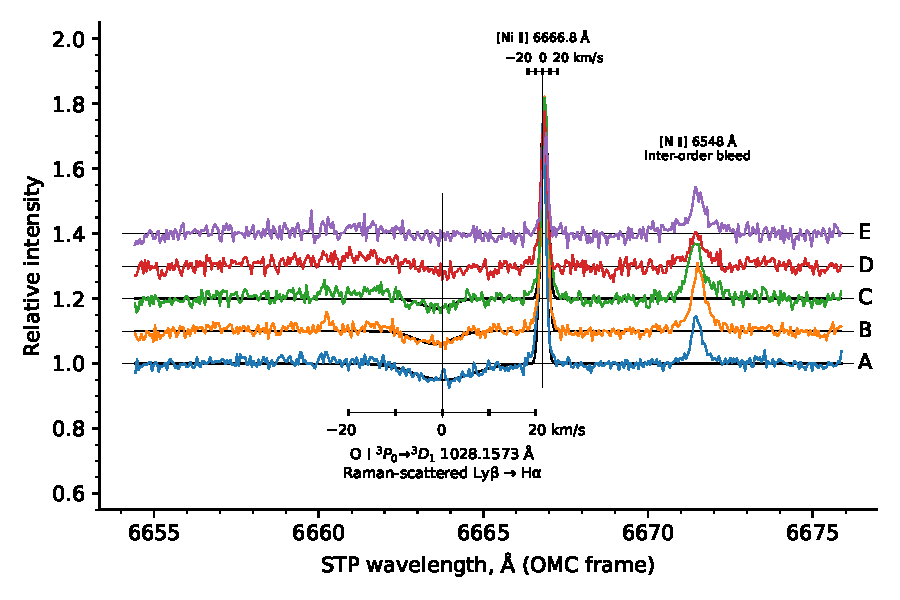
\includegraphics[width=\linewidth]{figs/order51-absorption-by-group}
  \caption{Keck HIRES spectra of Raman-scattered \ion{O}{1} absorption
    line for five regions in Orion~South.  Wavelengths are given on an
    air scale and in the rest-frame of the Orion Molecular Cloud, as
    defined by the peak velocity of \chem{^{13}CO}. }
  \label{fig:raman-keck}
\end{figure*}


\begin{table*}
  \caption{FUV/optical wavelength equivalencies for Raman scattering}
  \begin{tabular}{l R R R R R}\toprule
    % Transition & {UV wav, \AA{}} & {Freq, cm\textsuperscript{-1}} & {d Freq} & {Opt wav} & {Air wav}\\
    \text{Transition} & \text{A} & \text{B} & \text{C} & \text{D} & \text{E} \\
    \midrule
    H I \{1,2\}s \(\to\) 3p & 1025.72220 & 97492.283 & 0.000 & 6564.553248 & 6562.7406\\
    O I J = 0 \(\to\) 1 & 1028.15729 & 97261.383 & -230.900 & 6665.5868 & 6663.7469\\
    O I J = 1 \(\to\) 1 & 1027.43139 & 97330.100 & -162.183 & 6635.1951 & 6633.3630\\
    O I J = 1 \(\to\) 2 & 1027.43077 & 97330.159 & -162.124 & 6635.1691 & 6633.3370\\
    O I J = 2 \(\to\) 1 & 1025.76339 & 97488.369 & -3.914 & 6566.2400 & 6564.4269\\
    O I J = 2 \(\to\) 2 & 1025.76276 & 97488.429 & -3.854 & 6566.2141 & 6564.4010\\
    O I J = 2 \(\to\) 3 & 1025.76170 & 97488.530 & -3.753 & 6566.1706 & 6564.3575\\
    \bottomrule
  \end{tabular}

\end{table*}

\section{Discussion}
\label{sec:discussion}

The effective resolving power of the optical spectrograph is multiplied by 6.4 for the FUV domain.

The \ion{O}{1} lines should be in absorption in the spectrum seen by the Raman scatterers. 

\citet{Salgado:2016a} had found low dust cross-section in Orion Bar
PDR, but there are loopholes. First, they assume plane-parallel
geometry with exactly edge-on viewing angle, while in reality it is a
roughly cylindrical filament.  Second, they ignore scattering, see
\citet{Watson:1998a}.


Geometry of bar: in \citet{Henney:2005b} I pointed out that a
diverging cylindrical geometry is necessary to explain the sharp peak
in the [\ion{N}{2}] emissivity seen at the ionization front.  It has
been apparent since \citet{ODell:2000a} that the nebula contains many
bar-like features.

\bibliography{BibdeskLibrary}


\end{document}


\end{document}
%%% Local Variables:
%%% mode: latex
%%% TeX-master: t
%%% End:
